\documentclass[aspectratio=169]{beamer}
\usepackage{lmodern}
%\usetheme{Madrid}
%\usecolortheme{giantoak}
\newcommand*\oldmacro{}
\let\oldmacro\insertshorttitle
\renewcommand*\insertshorttitle{\oldmacro\hfill\insertframenumber\,/\,\inserttotalframenumber}
\usepackage[framemethod=tikz]{mdframed}

%\usepackage{beamerthemesplit}
\usepackage{textpos}
\usepackage{pgf}
%\logo{\pgfputat{\pgfxy(0,-.4)}{\pgfbox[right,base]{\includegraphics[height=1.0cm]{logo.jpg}}}}
%\newcommand{\nologo}{\setbeamertemplate{logo}{}}
\usepackage{booktabs}
\usepackage{graphicx}
\theoremstyle{principle}
\newtheorem*{principle}{Design Principle}


\titlegraphic{\includegraphics[width=1.0\paperwidth]{cool-wind-800px.jpg}}

\title{What are `political' numbers?}
%\author[Jeremy Kedziora]{Wind Data Science Team\\
%\small{Uptake}}
\date{}

\begin{document}

%{
%%\nologo
%\begin{frame}
%    \maketitle
%\end{frame}
%}
%pages 1-7, 8-9, 14-15.


{
%  \usebackgroundtemplate{
\includegraphics[width=1.0\paperwidth]{statistics-review.jpg}}
  \usebackgroundtemplate{
\includegraphics[scale=0.57]{statistics-review.jpg}}
  \begin{frame}[plain]
  
\begin{mdframed}[tikzsetting={draw=white,fill=white,fill opacity=0.6,draw opacity=0.4,
               line width=0pt},backgroundcolor=none,leftmargin=20,
               rightmargin=20,innertopmargin=4pt]
\begin{center}
\Huge \textbf{What are `political' numbers?}
\end{center}
\end{mdframed}

  \end{frame}
}

%%@@@@@@@@@@@@@@@@@@@@@@@@@@@@@@@@@@@@@@@@@@@@@@@@@
%\begin{frame}
%\vspace{1mm}
%\begin{center}
%\Huge \textbf{What are `political' numbers?}
%\end{center}
%
%\end{frame}
%
%%@@@@@@@@@@@@@@@@@@@@@@@@@@@@@@@@@@@@@@@@@@@@@@@@@
%\begin{frame}
%\vspace{12.5mm}
%\begin{center}
%\Huge \textbf{What are `political' numbers?}\\
%\bigskip
%\bigskip
%\textbf{Choices.}
%\end{center}
%
%\end{frame}

%@@@@@@@@@@@@@@@@@@@@@@@@@@@@@@@@@@@@@@@@@@@@@@@@@
\begin{frame}
\frametitle{Today}
\begin{itemize}
\item What jobs numbers do when related to politics;
\bigskip
\bigskip
\item Some characteristics of political numbers;
\bigskip
\bigskip
\item Dangers.
\end{itemize}

\end{frame}

%%@@@@@@@@@@@@@@@@@@@@@@@@@@@@@@@@@@@@@@@@@@@@@@@@@
%\begin{frame}
%\frametitle{Political numbers can be used for policy advocacy...}
%\begin{center}
%\textit{The numbers speak for themselves: Nearly 90\% of student loan debt relief will go to borrowers earning less than \$75,000; 85\% of the congressional Republicans’ tax cut went to taxpayers earning more than \$75,000.}\\
%\bigskip
%\hspace{70mm}$\sim$ White House tweet 28 August
%\end{center}
%\bigskip
%\begin{itemize}
%\item Suggestion is that loan forgiveness is aimed at the middle class while earlier tax cuts were aimed at the wealthy;
%\bigskip
%\bigskip
%\item[]\color{white} \href{https://www.washingtonpost.com/politics/2022/08/30/white-houses-tricky-comparison-between-student-loan-relief-gop-tax-cuts/}{\underline{To start}}: actual reference for loans is for individual income, for tax cuts is for household income.
%\end{itemize}
%
%\end{frame}

%@@@@@@@@@@@@@@@@@@@@@@@@@@@@@@@@@@@@@@@@@@@@@@@@@
\begin{frame}
\frametitle{Political numbers can be used for policy advocacy...}
\begin{center}
\textit{The numbers speak for themselves: Nearly 90\% of student loan debt relief will go to borrowers earning less than \$75,000; 85\% of the congressional Republicans’ tax cut went to taxpayers earning more than \$75,000.}\\
\bigskip
\hspace{70mm}$\sim$ White House tweet 28 August
\end{center}
\bigskip
\begin{itemize}
\item Suggestion is that loan forgiveness is aimed at the middle class while earlier tax cuts were aimed at the wealthy;
\bigskip
\bigskip
\item \href{https://www.washingtonpost.com/politics/2022/08/30/white-houses-tricky-comparison-between-student-loan-relief-gop-tax-cuts/}{\color{blue}\underline{To start}}\color{black}: actual reference for loans is for individual income, for tax cuts is for household income.
\end{itemize}

\end{frame}

%@@@@@@@@@@@@@@@@@@@@@@@@@@@@@@@@@@@@@@@@@@@@@@@@@
\begin{frame}
\frametitle{Political numbers can be related to electoral politics...}
\begin{center}
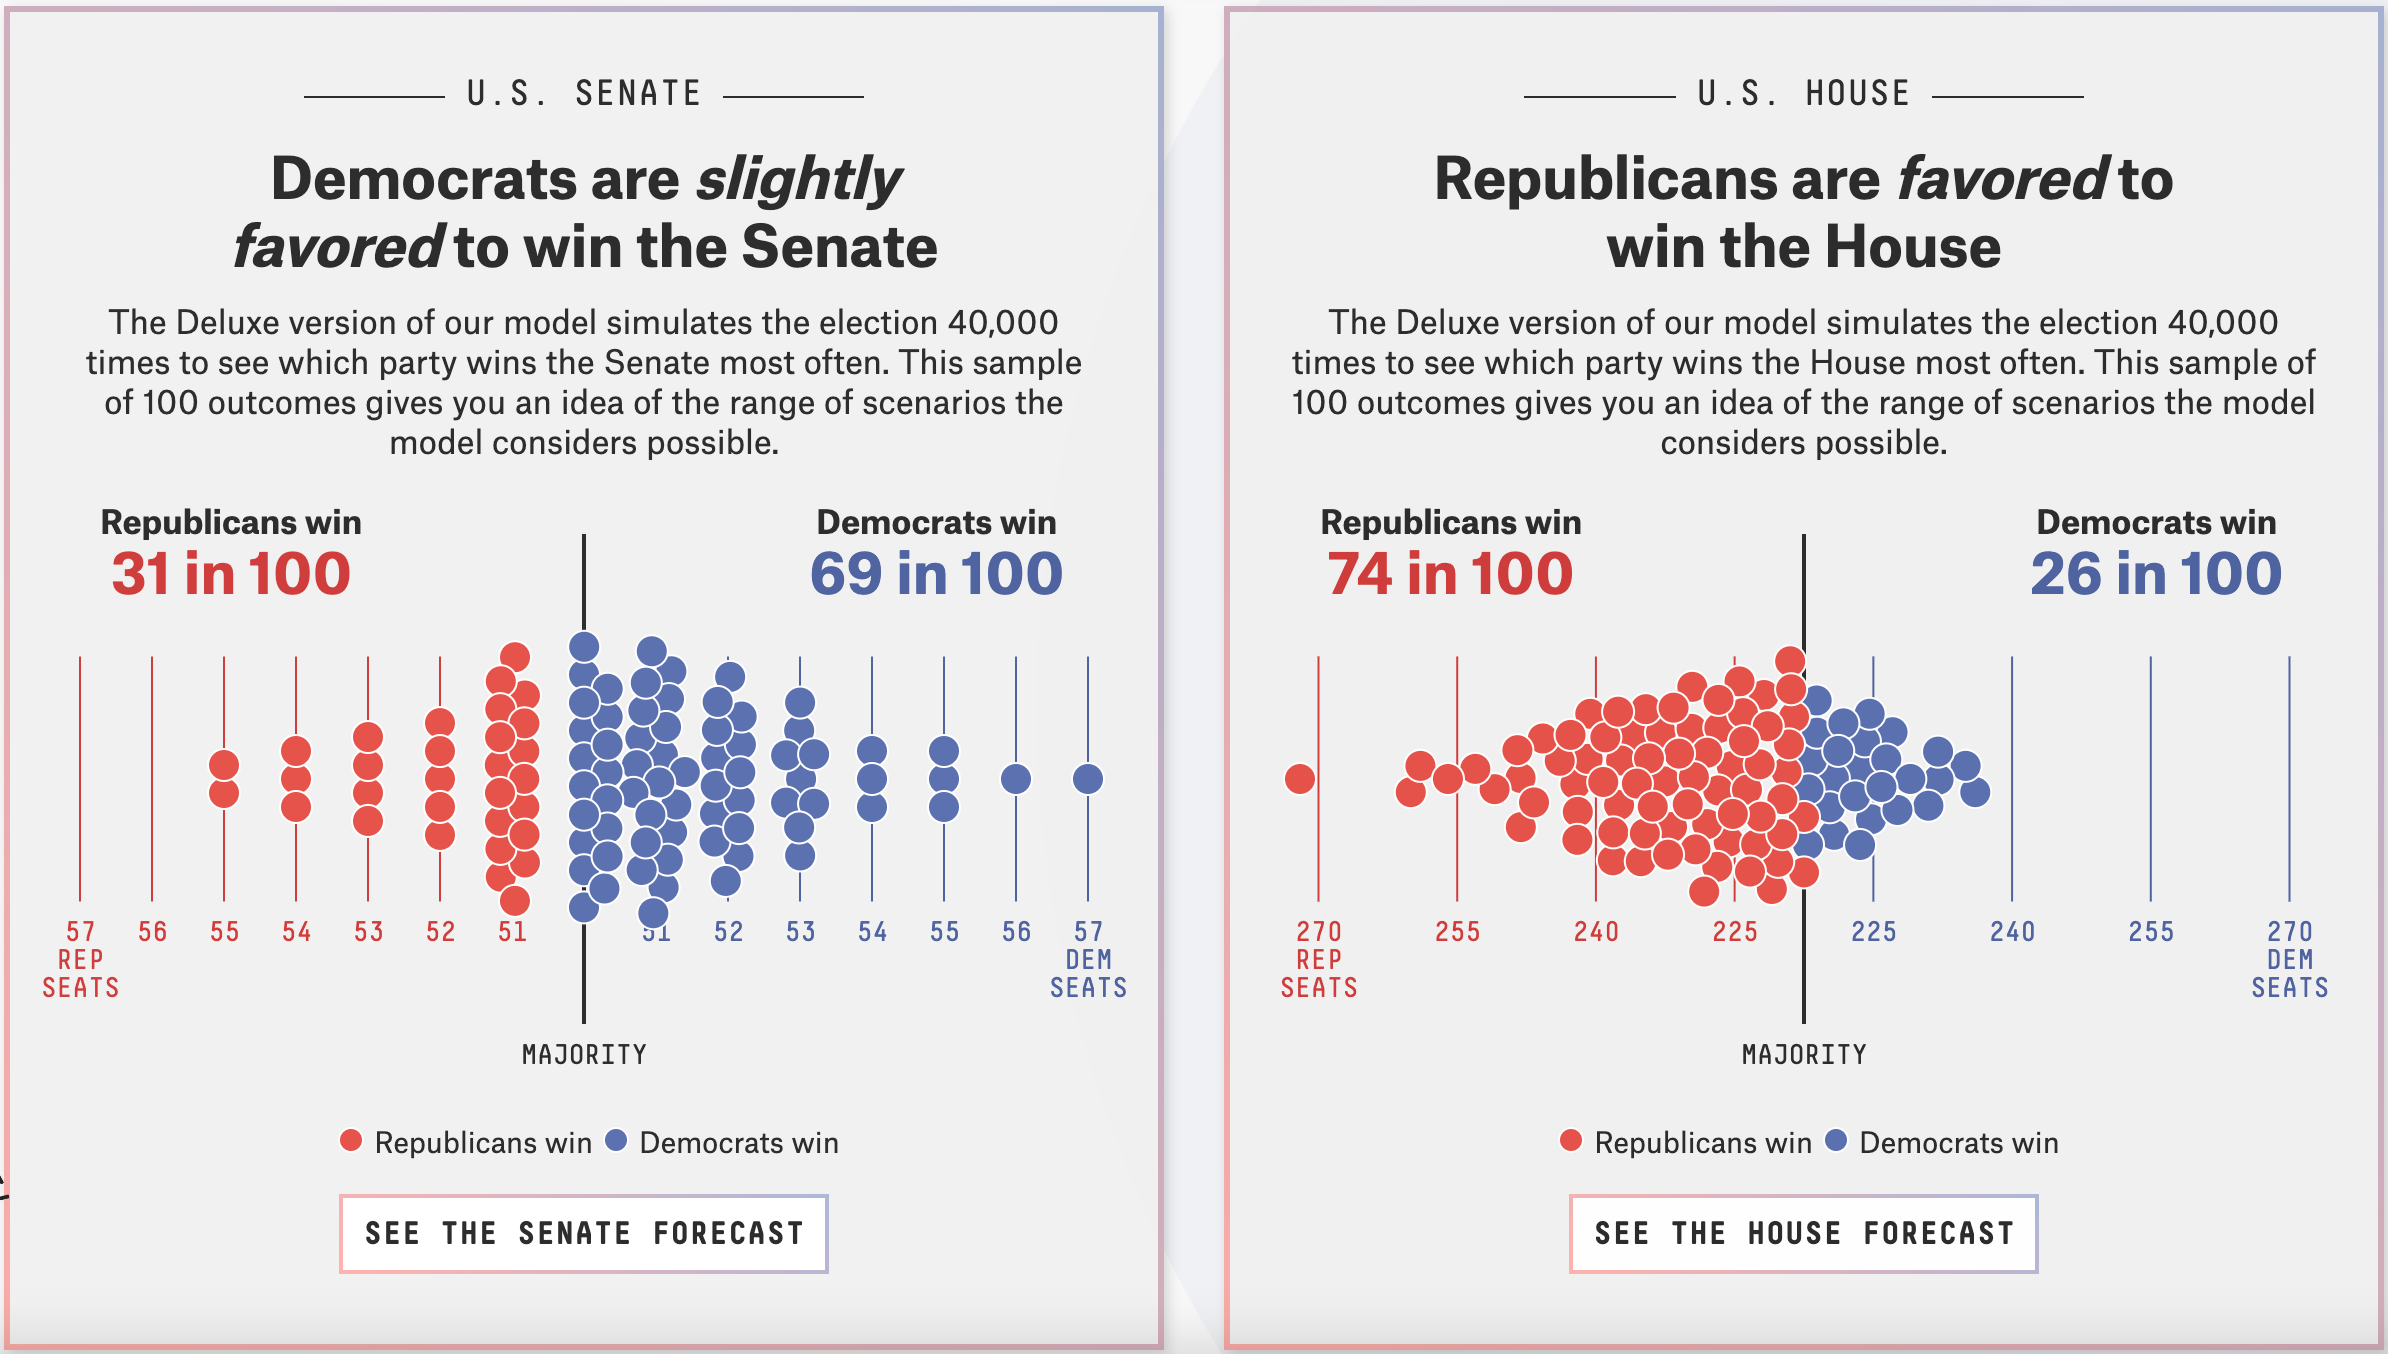
\includegraphics[scale=0.3]{538.png}
\end{center}

\end{frame}

%@@@@@@@@@@@@@@@@@@@@@@@@@@@@@@@@@@@@@@@@@@@@@@@@@
\begin{frame}
\frametitle{Political numbers can be about science...}
\begin{center}
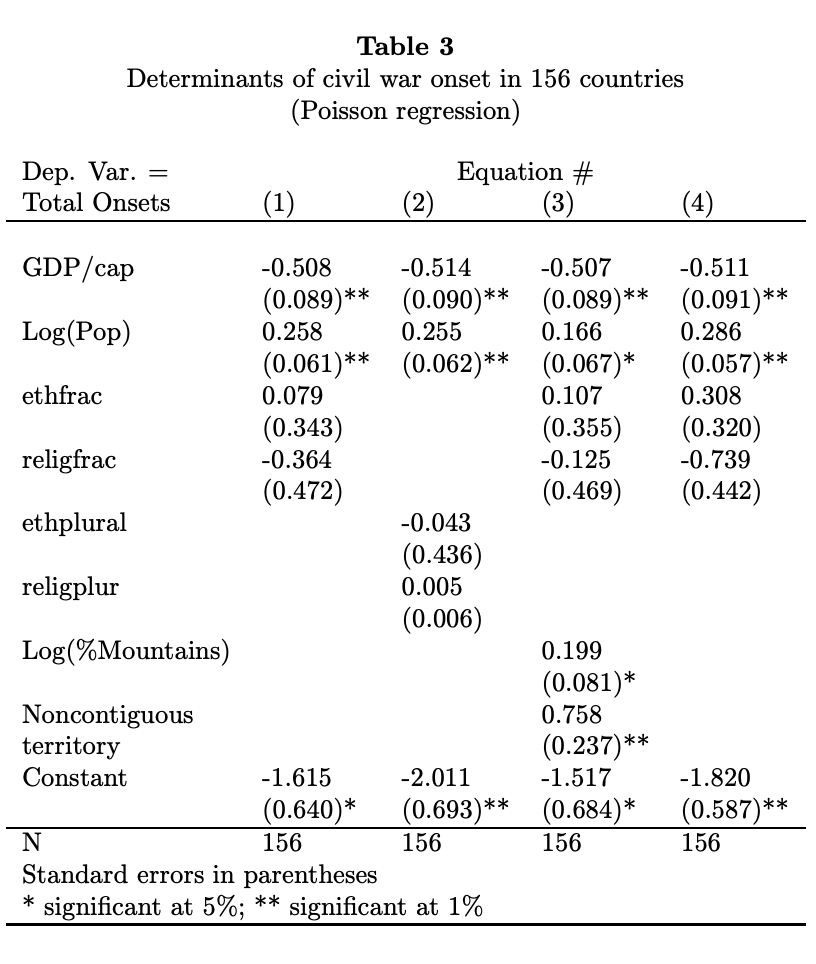
\includegraphics[scale=0.45]{f_and_l.png}
\end{center}

\end{frame}

%@@@@@@@@@@@@@@@@@@@@@@@@@@@@@@@@@@@@@@@@@@@@@@@@@
\begin{frame}
\frametitle{Three characteristics of political numbers:}
\begin{itemize}
\item They can be manipulated;
\bigskip
\bigskip
\bigskip
\item They create winners and losers;
\bigskip
\bigskip
\bigskip
\item They potentially involve agency.
\end{itemize}

\end{frame}


%@@@@@@@@@@@@@@@@@@@@@@@@@@@@@@@@@@@@@@@@@@@@@@@@@
\begin{frame}
\frametitle{Manipulation}
\begin{itemize}
\item How do we measure unemployment?
\begin{itemize}
\item \textbf{Decide} what concept to capture: need for jobs?  Supply of labor?  Demand for labor?
\item \textbf{Transform} this into something observable: people wanting work;
\item \textbf{Operationalize} by fixing inclusion criteria: older than 16, had a job previously, have looked in previous 4 weeks, and are available;
\end{itemize}
\bigskip
\bigskip
\item Definition of measurement $=$ definition of the problem and therefore a main avenue of political conflict;
\bigskip
\bigskip
\item What about those who...
\begin{itemize}
\item ...can get dangerous/demeaning/unpleasant jobs but don't;
\item ...could get part time but hold out for full time;
\item ...quit to find something better but are still searching;
\item ...can get a job but can't find child care to take a job;
\item ...have never worked but want to now.
\end{itemize}

\end{itemize}
\end{frame}

%@@@@@@@@@@@@@@@@@@@@@@@@@@@@@@@@@@@@@@@@@@@@@@@@@
\begin{frame}
\frametitle{Manipulation}
\begin{center}
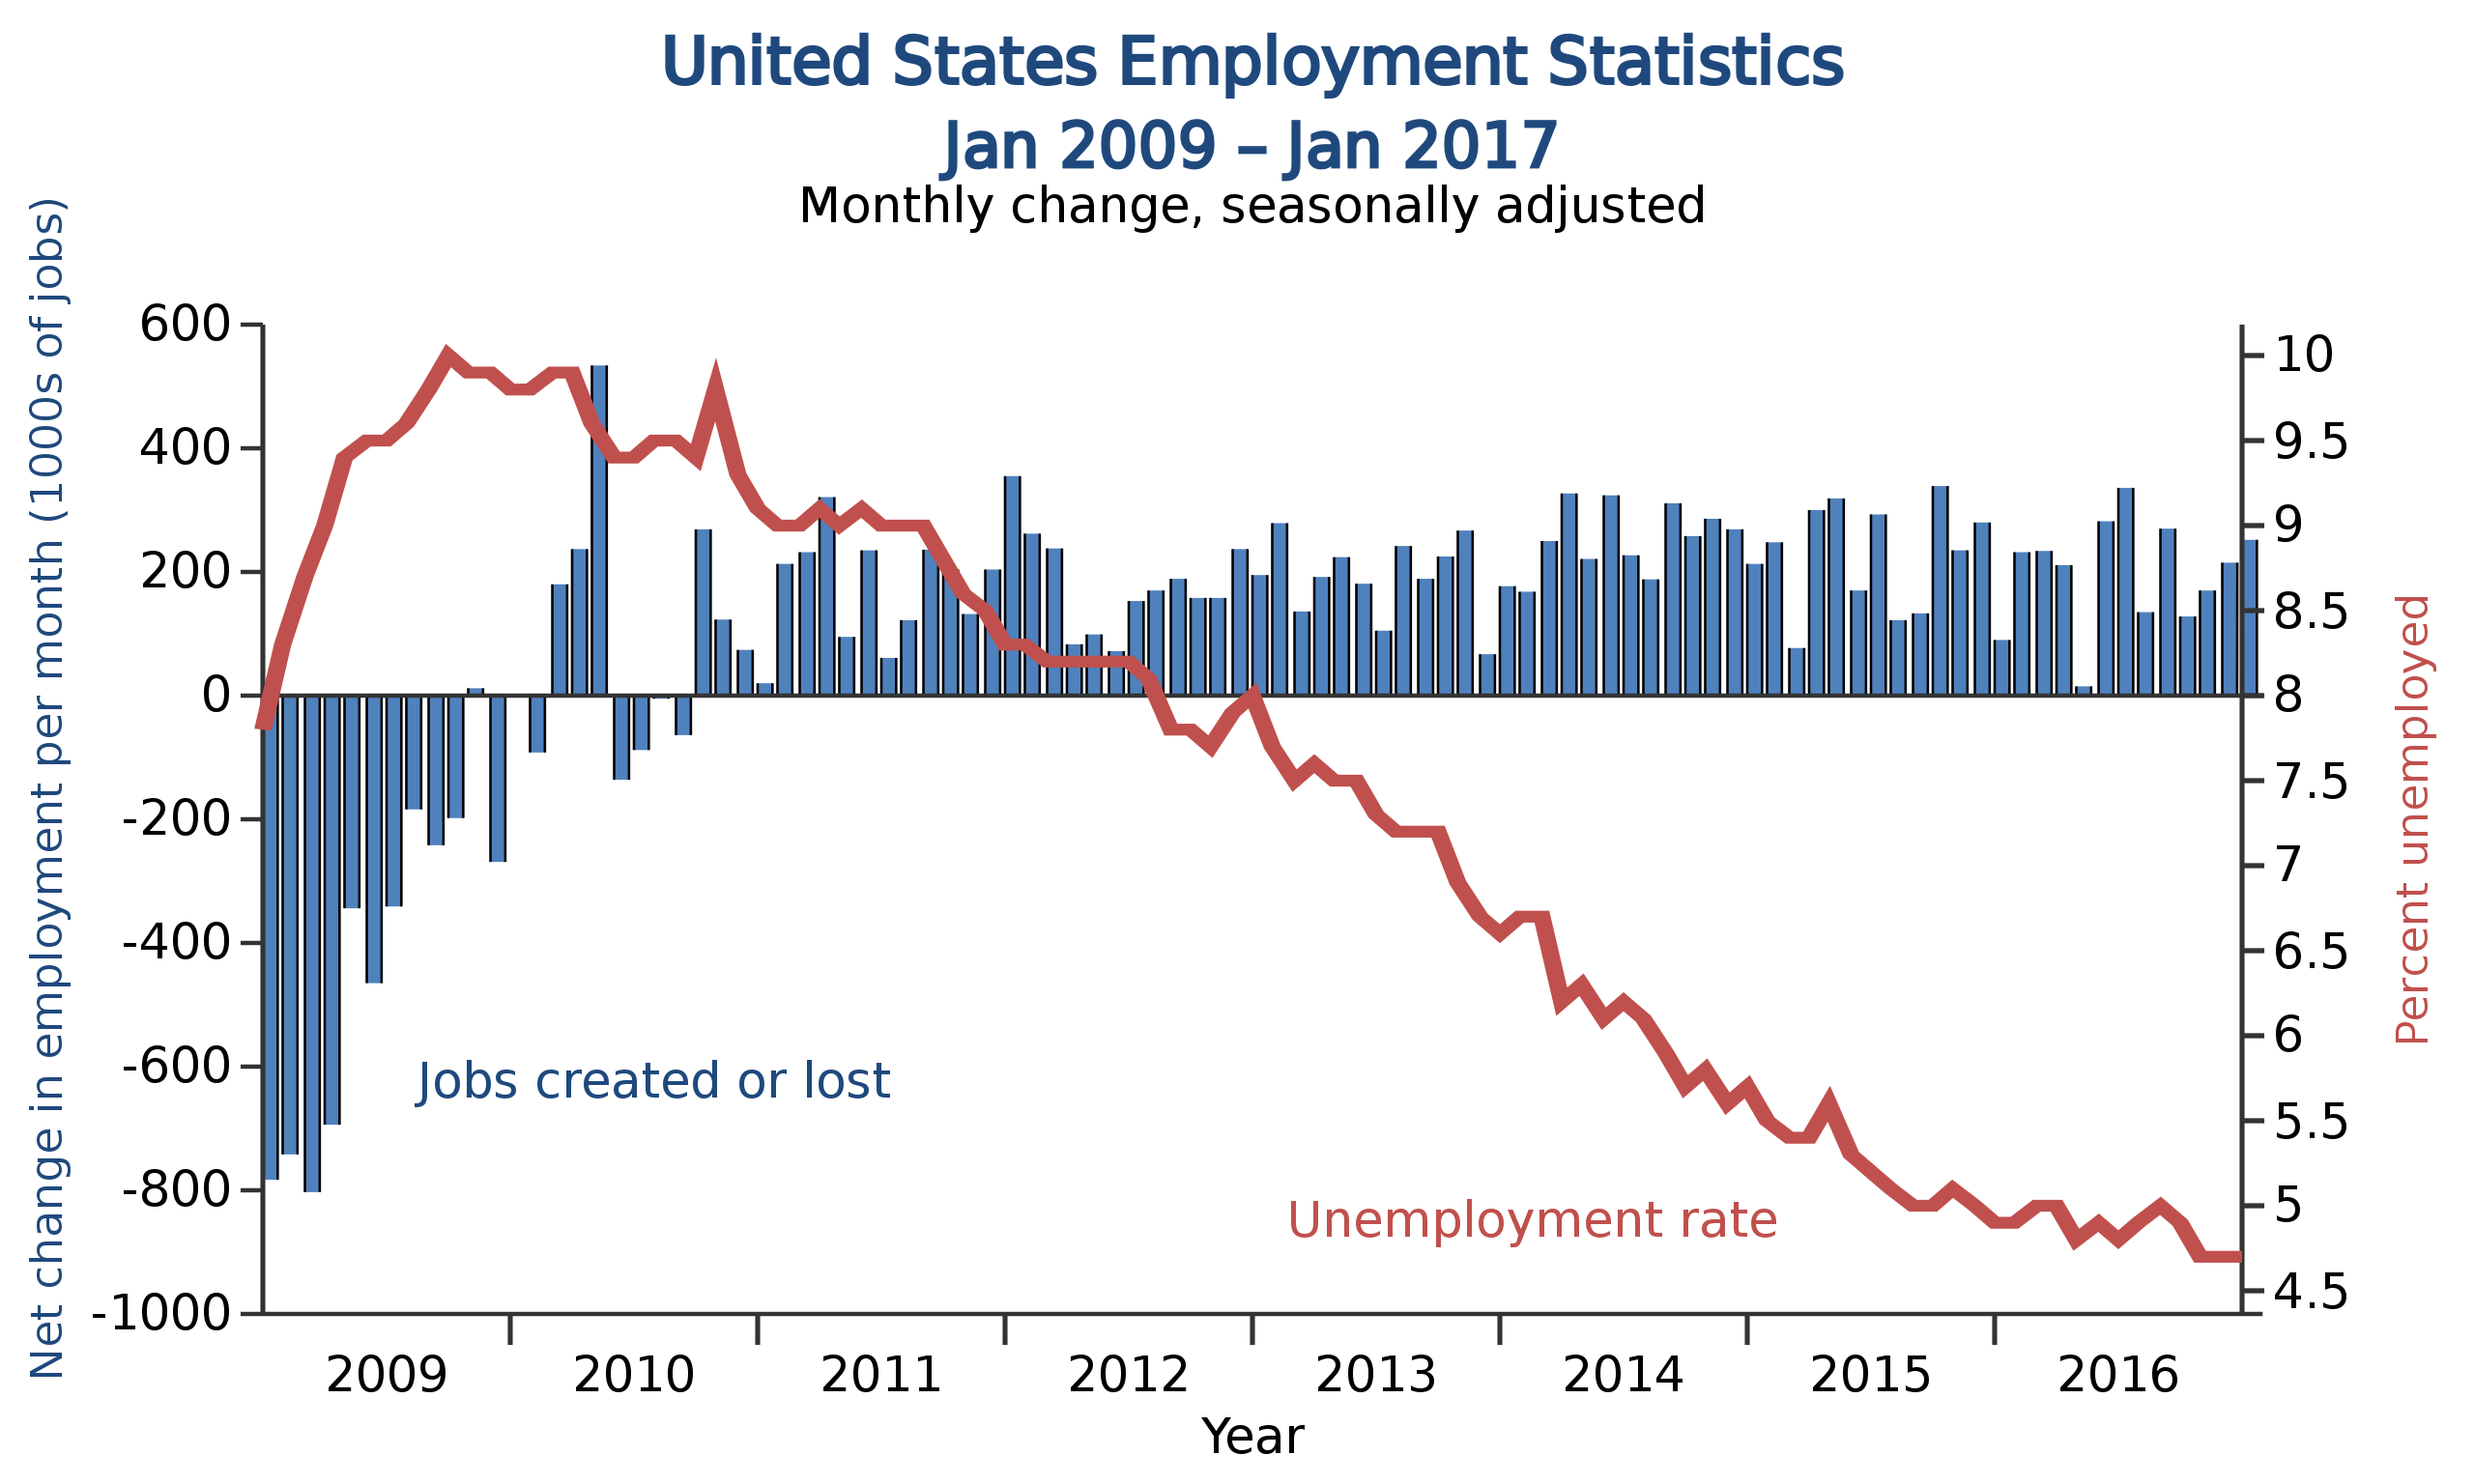
\includegraphics[scale=0.12]{unemployment.png}
\end{center}

\end{frame}

%@@@@@@@@@@@@@@@@@@@@@@@@@@@@@@@@@@@@@@@@@@@@@@@@@
\begin{frame}
\frametitle{Manipulation}
\begin{center}
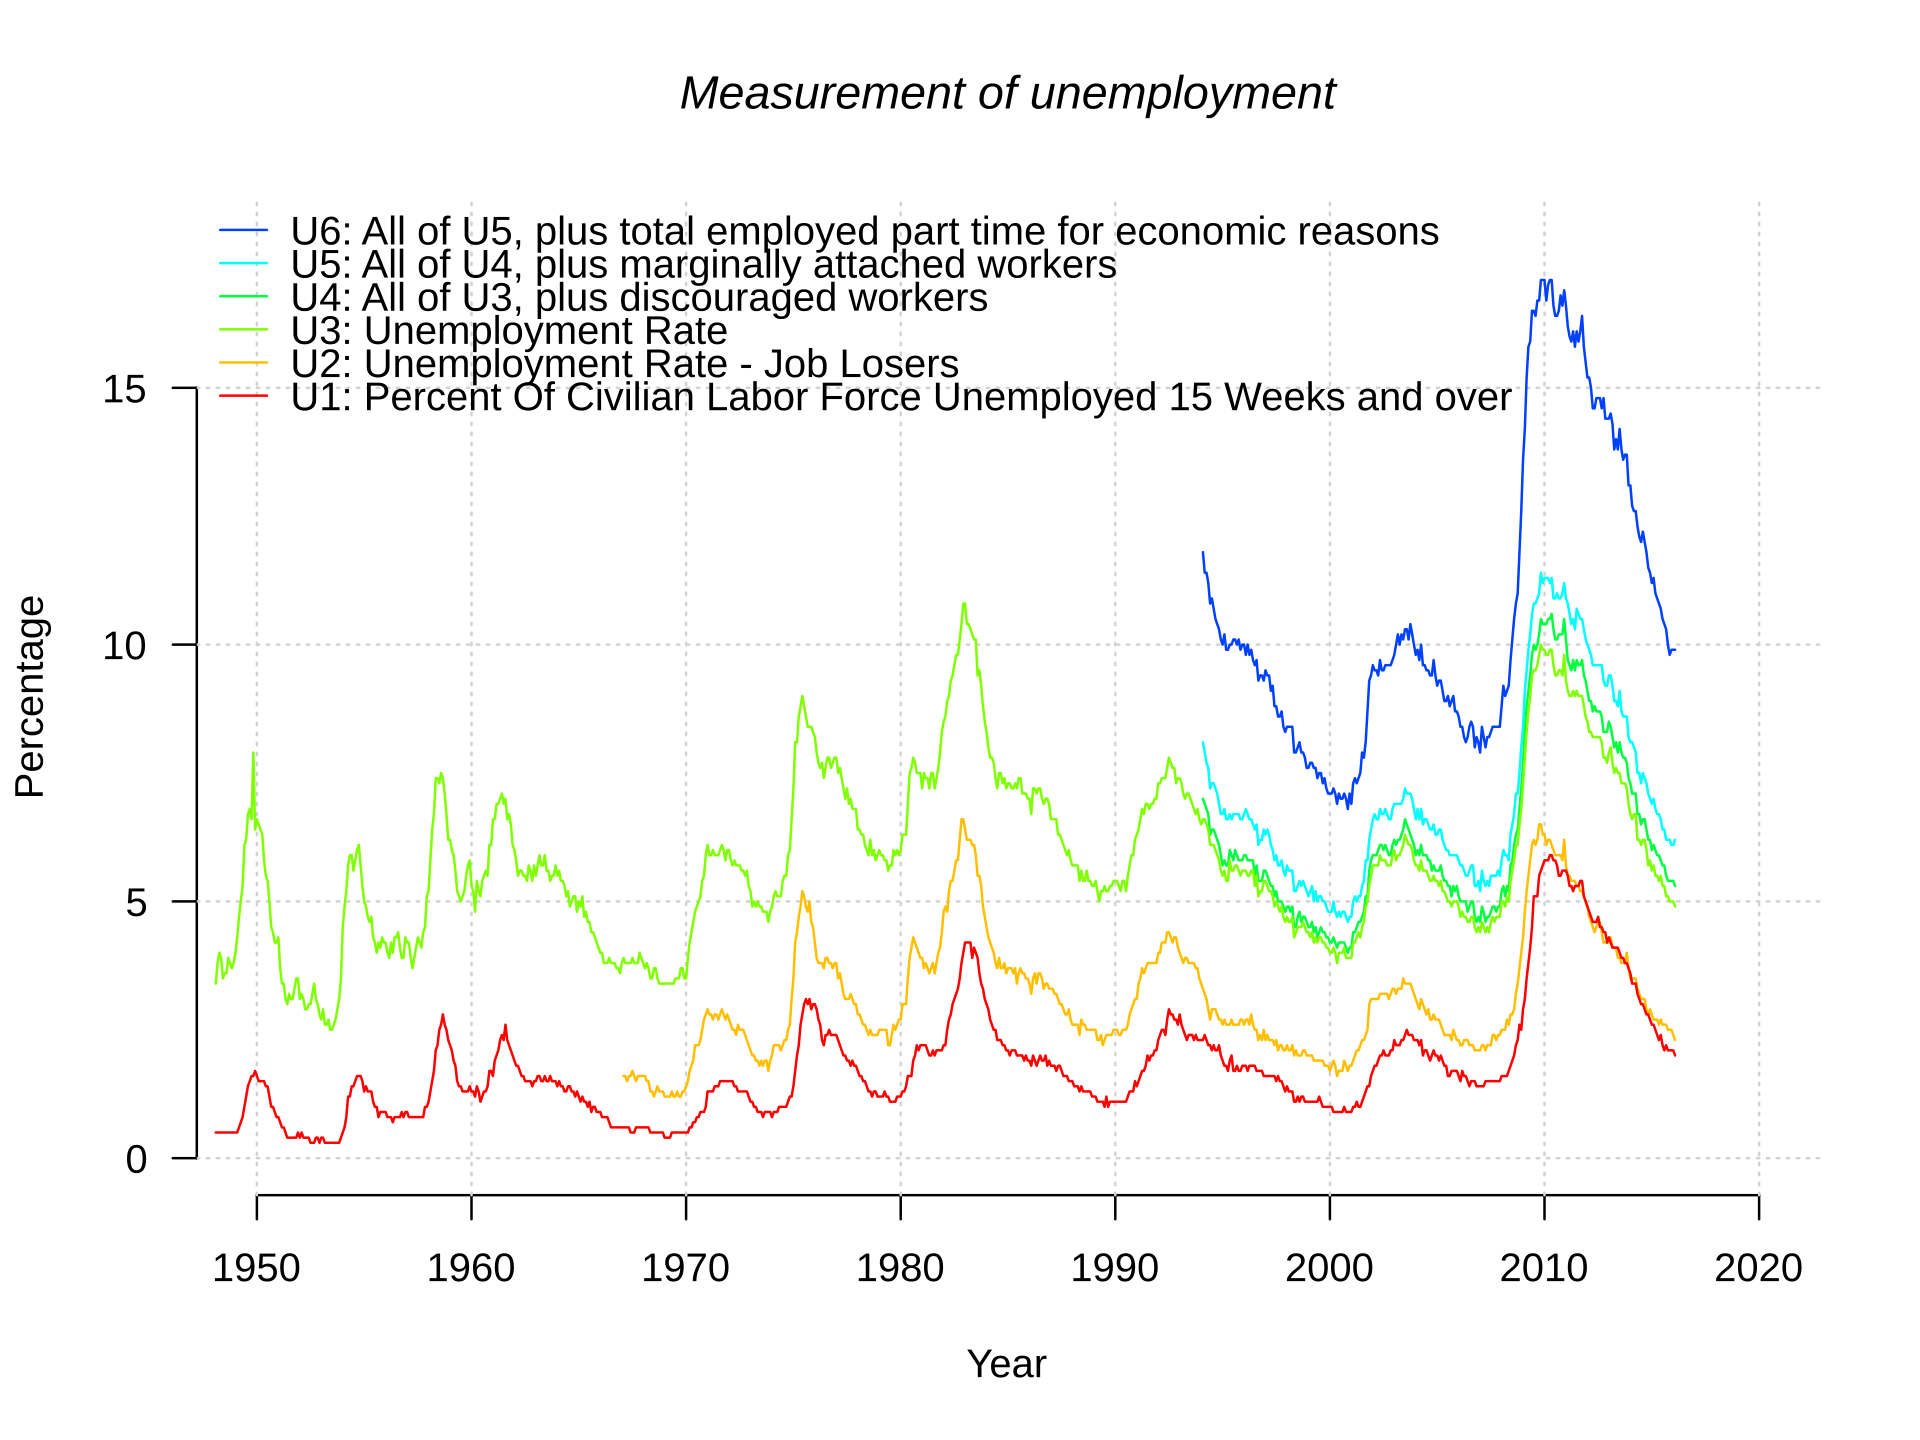
\includegraphics[scale=0.15]{unemployment_2.png}
\end{center}

\end{frame}

%@@@@@@@@@@@@@@@@@@@@@@@@@@@@@@@@@@@@@@@@@@@@@@@@@
\begin{frame}
\frametitle{Manipulation}

\begin{itemize}
\item How many public water systems are there in the US?
\bigskip
\bigskip
\item Public water system: $\geq$15 service connections or service to an average of $\geq$ 25 people for $\geq$ 60 days a year;
\bigskip
\bigskip
\item With this definition, over 148k;
\begin{itemize}
\item Community Water System;
\item Non-Transient Non-Community Water System;
\item Transient Non-Community Water System.
\end{itemize}
\end{itemize}

\end{frame}

%@@@@@@@@@@@@@@@@@@@@@@@@@@@@@@@@@@@@@@@@@@@@@@@@@
\begin{frame}
\frametitle{Manipulation}
\begin{itemize}
\item ``As answers to policy problems, the resolution numbers offer is nothing more than a human decision about how to count as"  (i.e. numbers $=$ metaphors);
\bigskip
\bigskip
\item Wrongful exclusion:
\begin{itemize}
\item Measurement assigns a difference but `actually' there is likeness;
\item Examples: unemployed, homelessness, grades, excess mortality during war;
\end{itemize}
\bigskip
\bigskip
\item Wrongful inclusion:
\begin{itemize}
\item Measurement assigns a likeness but `actually' there is difference;
\item Examples: generational cohorts, excess mortality during war (Iraq war deaths);
\end{itemize}
\end{itemize}
\end{frame}

%@@@@@@@@@@@@@@@@@@@@@@@@@@@@@@@@@@@@@@@@@@@@@@@@@
\begin{frame}
\frametitle{Creating winners and losers}
\begin{itemize}
\item Expertise and authority (e.g. Mitt Romney);
\bigskip
\bigskip
\item Recognition or assertion that something is widespread but unobserved (e.g. COVID);
\bigskip
\bigskip
\item Claim of clear boundaries (e.g. insurgency);
\bigskip
\bigskip
\item Creation of community (e.g. population).
\end{itemize}
\end{frame}

%@@@@@@@@@@@@@@@@@@@@@@@@@@@@@@@@@@@@@@@@@@@@@@@@@
\begin{frame}
\frametitle{Agency}
\begin{itemize}
\item \textbf{Strategic choice selection effects}--when observations are actors making choices the way they solve their optimization problems can have consequences for how they appear in the data;
\bigskip
\bigskip
\item \textbf{Observer effects}–people behave differently when observed (e.g. poll responses);
\bigskip
\bigskip
\item Using numbers where there is agency can create \textbf{self-fulfilling prophecy}--example, by counting people as part of a group, a policy may induce them to act as a group to then advocate for themselves;
\bigskip
\bigskip
\item Question: if DOJ Antitrust Division measures market concentration to decide whether to permit corporate mergers and acquisitions, how do you think this might affect how large companies lobby regarding the definition of their ``market"?
\end{itemize}
\end{frame}

%@@@@@@@@@@@@@@@@@@@@@@@@@@@@@@@@@@@@@@@@@@@@@@@@@
\begin{frame}
\frametitle{Artifacts and dangers...}
\begin{columns}
\begin{column}{0.5\textwidth}

\begin{itemize}
\item Numbers can reduce conflicts to a single dimension;
\begin{itemize}
\item e.g., if we only considered the energy density of fuel sources (versus cost or safety), we might draft policy to build more nuclear power plants...
\end{itemize} 
\bigskip

\item Numbers legitimize decisions;
\begin{itemize}
\item ...and sometimes mask the \textbf{political} nature of a decision;
\item For example: What is a ``safe number of organisms that could be discharged per cubic meter of water?"
\end{itemize}
\end{itemize}

\end{column}
\begin{column}{0.5\textwidth}
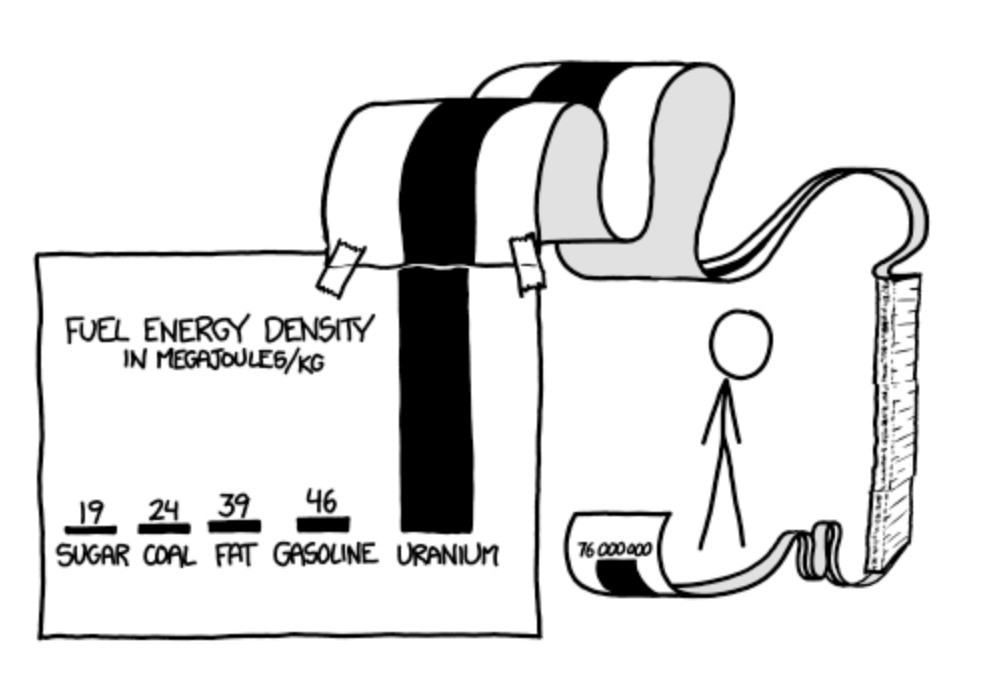
\includegraphics[scale=0.4]{energy.png}
\end{column}
\end{columns}

\end{frame}

%@@@@@@@@@@@@@@@@@@@@@@@@@@@@@@@@@@@@@@@@@@@@@@@@@
\begin{frame}
\frametitle{Artifacts and dangers...}
\begin{columns}
\begin{column}{0.5\textwidth}

\begin{itemize}
\item Numbers can reduce conflicts to a single dimension;
\begin{itemize}
\item e.g., if we only considered the energy density of fuel sources (versus cost or safety), we might draft policy to build more nuclear power plants...
\end{itemize} 
\bigskip

\item Numbers legitimize decisions;
\begin{itemize}
\item ...and sometimes mask the \textbf{political} nature of a decision;
\item For example: What is a ``safe number of organisms that could be discharged per cubic meter of water?"
\end{itemize}
\end{itemize}

\end{column}
\begin{column}{0.5\textwidth}
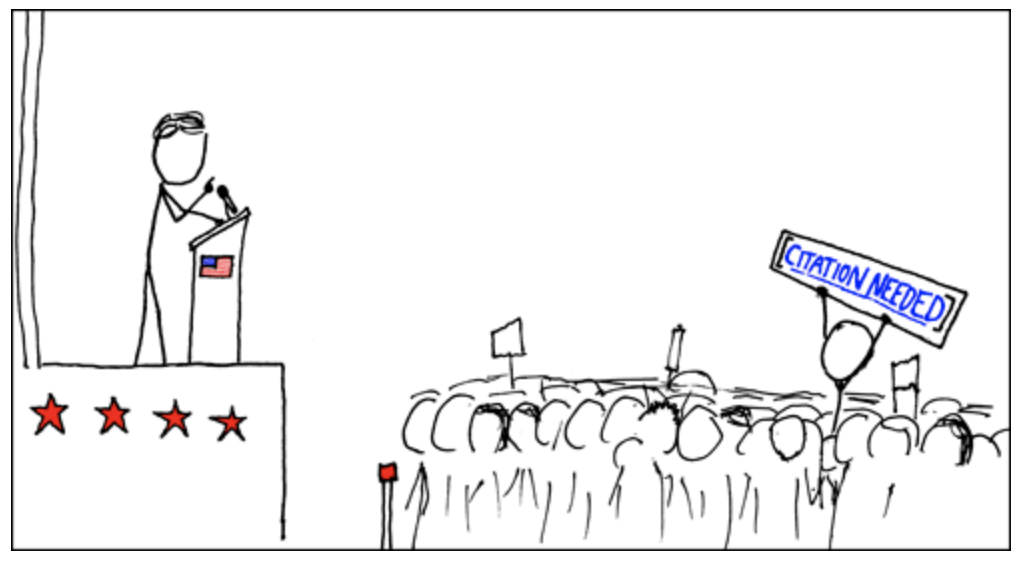
\includegraphics[scale=0.4]{speech.png}
\end{column}
\end{columns}

\end{frame}

%@@@@@@@@@@@@@@@@@@@@@@@@@@@@@@@@@@@@@@@@@@@@@@@@@
\begin{frame}

\begin{center}
\Huge\textbf{Why should we care?}\\
\bigskip
\bigskip
\large Building numbers to measure generally involves choices over how to count and who wins.  The power to choose is the power to control.\\
\end{center}

\end{frame}

%ADD ONE MORE EXAMPLE

\end{document}






